\documentclass[singlespacing, latexmargins]{ludis}

% % custom packages by Peteris Ratnieks
% \usepackage{booktabs}
% \usepackage[normalem]{ulem}
% \usepackage{amsmath}
% \usepackage{amsfonts}
% \usepackage{amssymb}
% \usepackage{mathabx}
% \usepackage{upgreek}
% \usepackage{hyperref}
% \usepackage{mathtools}
% \usepackage{graphicx}
% \usepackage{float}
% \usepackage{wrapfig}
% \usepackage{caption}
% \usepackage{subcaption}
% \usepackage{listings}
% %\usepackage{fullpage}
% % custom definitions
% \DeclarePairedDelimiter\abs{\lvert}{\rvert}%
% \DeclarePairedDelimiter\norm{\lVert}{\rVert}%
% \makeatletter
% \let\oldabs\abs
% \def\abs{\@ifstar{\oldabs}{\oldabs*}}
% \let\oldnorm\norm
% \def\norm{\@ifstar{\oldnorm}{\oldnorm*}}
% \makeatother
% \lstset{numbers=left,
    % stepnumber=1,
    % firstnumber=1,
    % numberfirstline=true
% }
% \lstinputlisting[language=Python, firstline=2, lastline=22]{code.py}

% XeLaTeX atbalsts tiek pieslēgts ar šādām pakotnēm:
\usepackage{fontspec}
\usepackage{xunicode}
\usepackage{xltxtra} %

% Valodu atbalsts
\usepackage{polyglossia}
\setdefaultlanguage{latvian}
\setotherlanguages{english,russian}

% Fonti -- var rakstīt sistēmas fontu nosaukumus
% \setmainfont[Mapping=tex-text]{Times New Roman}
% \setsansfont[Mapping=tex-text]{Arial}
% \newfontfamily\russianfont{Times New Roman}

\usepackage{multirow}

\usepackage{hyperref}


% \def\r{\mathbb{R}}
% \def\c{\mathbb{C}}
% \def\k{\mathbb{K}}
% \def\z{\mathbb{Z}}
\def\n{\mathbb{N}}
% \def\co{\mathsf{co}}

\def\m{\mathcal{M}}
\def\k{\mathcal{K}}
\def\a{\mathcal{A}}

\def\sumin{\sum_{i=1}^n}
\def\sumon{\sum_{i=0}^n}
\def\suminf{\sum_{i=1}^\infty}
\def\ppt{\textsf{PPT}}
\def\oi{\{0,1\}}
% \def\p{\textsf{P}}

% \def\svp{\textsf{SVP} }
% \def\cvp{\textsf{CVP}}
% \def\svpg{\textsf{SVP$_\gamma$} }
% \def\cvpg{\textsf{CVP$_\gamma$} }
% \newcommand{\bra}[2]{\langle #1,#2 \rangle} 


\fakultate{Fizikas un Matemātikas}
\nodala{Matemātikas}
\nosaukums{Vai blokķēdi var izmantot kā trešo pusi godīgas apmaiņas problēmā.}
\autors{Pēteris Ratnieks}
\gads{2017}



\begin{document}

\maketitle

\begin{abstract-lv}
    not implemented

    \keywords{blokķēde, godīga apmaiņa, virtuālā nauda}
\end{abstract-lv}

\begin{abstract-en}
    not implemented

\keywords{blockchain, fair exchange, virtual currency}
\end{abstract-en}

\tableofcontents

\specnodala{Apzīmejumi}
\begin{description}
    \item[\ppt] Varbūtisks algoritms
    \item[$\m$]Ziņojumu telpa
    \item[$\k$]Atslēgu telpa
    \item[$Gen$]Atslēgu ģenerēšanas algoritms
    \item[$Enc$]Šifrēšanas algoritms
    \item[$Dec$]Atšifrēšanas algoritms
    \item[$Sig$]Parakstīšanas algoritms
    \item[$Ver$]Paraksta pārbaudīšanas algoritms
    \item[$P(A|B)$]Notikuma $A$ varbūtība, ja ir izpildījies notikums $B$
    \item[$x \leftarrow \a$]$x$ pieņem vērtību, kuru izdod varbūtiskais algoritms $\a$
    \item[$\oi^n$] Nuļļu un vieninieku virkņu telpa garumā $n$ 
    \item[$\oi^*$]Patvaļīga garuma nuļļu un vieninieku virkņu telpa
    \item[$\mathbf{1}^n$]Vieninieku virkne garumā $n$ (drošuma parametrs)
    \item[$U(X)$] Gadījuma lielums, kas raksturo vienmērīgu sadalījumu pār kopas $X$ elementiem
\end{description}


\specnodala{Ievads}
Tirdzniecība interneta vidē gūst arvien lielāku popularitāti. Ar to saistītas arī vairākas problēmas attiecībā pret godīgu apmaiņu starp divām savstarpēji neuzticīgām pusēm. Pieņemsim, ka Alise un Bobs abi vēlas parakstīt elektronisku dokumentu, bet katrs no viņiem otram neuzticās tapēc Alise nesūtīs Bobam savu parakstu pirms Bobs neatsūtīs viņai savējo un otrādi. Tādējādi viņi nekad neapmainīsies ar parakstiem, turklāt ir pierādīts, ka bez trešās puses iejaukšanās nav iespējams sasniegt stingri godīgu apmaiņu. \cite{pagnia99}
Ir piedāvāti dažādi problēmas risinājumi ar dažādām trešajām pusēm, bet ņemot vērā nesenos sasniegumus kriptovalūtu jomā uzskatu par nepieciešamu izpētīt risinājumus, kas trešās puses lomā novieto blokķēdi. 

Lai labāk saprastu godīgas apmaiņas problēmu norādīsim neformālu definīciju un aplūkosim vēl vienu piemēru.  
An exchange is fair if at the end of the exchange, either each player
receives the item it expects or neither player receives any additional
information about the other's item. \cite[p.~8]{asokan98}

Asokan, N. 1998. Fairness in electronic commerce . Ph. D. thesis, University of Waterloo.

Godīga apmaiņa ir tāda, ka pēc tās izpildes katrs dalībnieks iegūst ziņojumu, ko sagaidīja, vai arī neviens no dalībniekiem neguva papildus informāciju par citiem ziņojumiem.[Asokan 1998, p. 8]

Blokķēde (ķēde) ir datu struktūra līdzīga saistītam sarakstam, bet katrā posmā tiek ierakstīta iepriekšējā posma hash vērtība, tādējādi tajā nav iespējams ievietot jaunu posmu pa vidu, bet tos var pievienot tikai ķēdes galā. 
Tipiskākais ķēdes lietojums ir decentralizētās elektroniskās valūtās, lai novērstu iespēju melot par ķēdes vēsturi. 
Šī darba kontekstā ar ķēdi sapratīsim publisku datu bāzi, kurā ir iespējams rakstīt, bet nav iespējams mainīt vēsturi.
Pieņemsim, ka katrs ķēdes posms sastāv no vairākiem ierakstiem un katram ierakstam ir autors.
Lai izveidotu jaunu ierakstu jāizveido operācija uz kuras autors uzliek parakstu.

Ir pierādīts, ka atrisināt godīgas apmaiņas probēmu patvaļīgiem ziņojumiem ir neiespējami sistēmā kurā trūkst trešās puses. 
Problēmu var atvieglot pieļaujot trešās puses esamību un uzliekot ierobežojumus uz apmaināmajiem ziņojumiem.
Tiks aplūkots gadījums kur trešās puses lomā ir ķēdes.
Ziņojumi ir attiecīgo ķēžu operācijas ar derīgu parakstu.
Aprakstošais algoritms pārbauda paraksta derīgumu pret operāciju. 

Interneta forumos ir aprakstīts algoritms, kas pieļauj valūtu apmaiņu starp divām blokķēdēm.
Tā kā ir divas ķēdes ir arī divas operācijas un tiek panākts, lai izpildītos abas operācijas, vai arī neizpildītos neviena.
Varētu teikt, ka iesaistītās puses ir apmainījušās ar parakstītām ķēdes operācijām.
Šajā darbā tiks aplūkots kādas īpašības piemīt ķēdei, kā trešajai pusei, godīgas apmaiņas problēmā, kādi ierobežojumi piemīt operācijām kā arī formāli aprakstīts minētais algoritms un meklēts vispārīgāks teorētisks rezultāts, kas balstītos uz līdzīga principa.




\chapter{Teorijas apskats}
Vispirms tiek uzskaitītas kriptogrāfijas definīcijas publisko atslēgu kriptogrāfijas kontekstā. 
Tiek padziļināti aplūkota godīgas apmaiņas problēma un tās praktiskā nozīme.
Kā jāuzstāda problēma, lai uz ķēdes varētu veikt godīgu apmaiņu.
Tiek aprakstīti fundamentālie kritēriji, kuri izpildās jebkurai digitālai valūtai.
Kāpēc izkliedētas skaitļošanas sistēmas ir drošas.
Beigās tiek aplūkotas galvenās idejas, uz kurām balstās ķēde.


\section{Kriptogrāfijas definīcijas}
Šajā nodaļā tiek konspektēts minimālais kriptogrāfijas daudzums, lai darbs būtu uztverams, tomēr padziļinātas zināšanas ir ieteicamas un to iegūšana tiek atstāta lasītāja ziņā. Definīcijas un atsevišķi skaidrojumi tiek ņemti no\cite{pass10}.

Par \textbf{kriptosistēmu} sauc kopu $(\m, \k, Gen, Enc, Dec)$, kur
\begin{description}
    \item[$\m$]Ziņojumu telpa
    \item[$\k$]Atslēgu telpa
    \item[$Gen$]Atslēgu ģenerēšanas algoritms
    \item[$Enc$]Šifrēšanas algoritms
    \item[$Dec$]Atšifrēšanas algoritms
\end{description}

Par asimetrisku, jeb publisko atslēgu kriptosistēmu sauc tādu, kurai atslēgu telpa sastāv no pāriem $(k_p, k_s)$, kur $k_p$ ir publiskā atslēga un $k_s$ ir slepenā atslēga. Šajās sistēmās šifrēšanas algoritmam ir atļauts publisko atslēgu, bet atšifrēšanas algoritmam privāto. Turpmāk tiks runāts tikai par asimetriskām kriptosistēmām.

\textbf{Varbūtisks algoritms}, jeb varbūtiska polinomiālā laikā ierobežota Tjūringa mašīna (Probabilistic polynomial-time Turing machine (\ppt)) ir Tjūringa mašīna kurai papildus ievaddatu lentei ir dota lente, kura pēc katra soļa padod mašīnai jaunu gadījuma skaitli. Ātrdarbība tiek novērta no apakšas pieņemot, ka jebkuriem ievaddatiem tiks uzģenerēti tādi gadījuma skaitļi, kas liks algoritmam darboties pēc iespējas ilgāk. Algoritmu sauc par \textbf{efektīvu}, ja eksistē tāds polinoms $P$, ka jebkuram ievaddatu izmēram $n$ tas apstājas ātrāk kā $P(n)$ soļos. Varbūtiska algoritma rezultāts ir gadījuma lielums.

Varbūtisks algoritms $\a$ \textbf{aprēķina} funkciju $f$, ja
$$ \forall x : \quad P[\a(x) = f(x)] = 1 $$
Praksē tiek izmantoti arī algoritmi, kas retos gadījumos kļūdās, bet šī varbūtība ir tik maza, ka to var neņemt vērā.

Kriptosistēmu sauc par efektīvu, ja izpildās īpašības:
\begin{enumerate}
    \item $k \leftarrow Gen(1^n)$ ir \ppt, kas izveido atslēgu $k$ jebkurai $n\in\n$ vērtībai.
    \item $c \leftarrow Enc_k(m)$ ir \ppt, kas izveido šifrtektstu $c$ jebkurai atslēgai $k$ un ziņojumam $m$.
    \item $m \leftarrow Dec_k(c)$ ir \ppt, kas dotam $k$ atšifrē ziņojumu $c$.
    \item Izpildās īpašība, ka visiem ziņojumiem tiek atšifrēts tas pats kas tika nošifrēts.
        $$ \forall n\in\n, m\in\m \quad P[k\leftarrow Gen(1^n): Dec_k(Enc_k(m)) = m] = 1 $$
\end{enumerate}

Par \textbf{pretinieku} sauc \ppt{}  kurš kā ievaddatus saņem kriptosistēmu, publisko atslēgu un drošuma parametru $1^n$.

Jebkurai kriptosistēmai prasa, lai no dotiem $m\in\m$ un $k\in\k$ būtu iespējams efektīvi ģenerēt šifrtekstu $c$. Kā arī, lai no jebkura $c$ nevarētu noskaidrot $k$ vai $m$.

Par \textbf{vienvirziena funkciju} $f$ sauc tādu, kurai eksistē \ppt{} $\mathcal{C}$ kas aprēķina $f$, bet neeksistē \ppt{} $\a$ kuram 
$$ \forall y \in \text{Ran}(f): P[f(\a(y)) = y] = 1 $$
Vispārīga kriptogrāfijas teorija daudz balstās uz vienvirziena funkcijām un tām ir smalkāks iedalījums, bet dotajai definīcijai ir maza teorētiska vērtība.

Par jaucējfunkciju (hash function) sauc vienvirziena funkciju $h: \oi^* \to \oi^n$, kurai ir izpildās noturība pret sadursmēm. 
\begin{equation*}
    P[x, y \leftarrow \a : h(x) = h(y)] = 0
\end{equation*}
kur $\a$ ir pretinieks un $x\neq y$.

Par \textbf{parakstu sistēmu} sauc kortežu $(\m, \k, Gen, Sig, Ver)$ kuram izpildās
\begin{equation*}
    \forall m \in \m \;:\; P[k \leftarrow Gen: Ver_k(m, Sig_k(m))=\t] = 1
\end{equation*}
Šeit $\m$ ir ziņojumu telpa, $\k$ ir atslēgu telpa, $Gen$ ir atslēgu ģenerēšanas algoritms, $Sig$ ir parakstīšanas algoritms un $Ver$ ir paraksta pārbaudīšanas algoritms. Līdzīgi, kā kriptosistēmu gadījumā $k$ sastāv no slepenās atslēgas $k_s$, kuru izmanto parakstītājs un publiskās atslēgas $k_p$, kuru izmanto paraksta pārbaudei. Algoritma $Ver$ vērtību apgabals sastāv no divām vērtībām \textemdash{} derīgs $\t$ un nederīgs $\f$.

Par \textbf{parakstītu ziņojumu} sauc pāri $(m, s)$, kur $m\in \m$ ir ziņojums, bet $s$ ir paraksts. Atslēgu $k$ sauc par parakstītāju. Parakstītu ziņojumu $(m,s)$ sauc par derīgu, ja $Ver(m,s) =\t$.

Parakstu sistēmu sauc par drošu, ja
\begin{equation*}
    P[k \leftarrow Gen; (m,s) \leftarrow \a (k_p)\;:\; m\ni Q \wedge Ver_k(m,s) =\t] = 0
\end{equation*}
kur $\a$ ir pretinieks kuram pieejams orākuls, kas saņemot $m$ atbild ar $Sig_k(m)$, bet $Q$ ir saraksts ar jautājumiem, kuri tika uzdoti orākulam.\cite[p.~135]{pass10}

No kriptosistēmas $(\m', \k', Gen', Enc, Dec)$ un jaucējfunkcijas $h$ var uzkonstruēt parakstu sistēmu $(\m, \k, Gen, Sig, Ver)$
\begin{align*}
    & \m = \m' \\
    & \k = \left\{ (k_s, k_p) | (k_p, k_s) \in \k' \right\} \\
    & Gen = Swap(Gen') \\
    & Sig(m) = \big(m, Enc_k(h(m))\big)  \\
    & Ver(m,s) =
    \begin{cases}
        \t, &\text{ja}\; h(m) = Dec_k(s) \\
        \f, &\text{citādi}
    \end{cases}
\end{align*}
Ievēro, ka parakstu sistēmas privātā atslēga ir kriptosistēmas publiskā un otrādi, tapēc no kriptosistēmas papildus nepieciešams nosacījums, ka no slepenās atslēgas un nošifrētiem ziņojumiem nevar izskaitļot publisko atslēgu.


\section{Godīga apmaiņa}
Aplūkosim Alisi un Bobu. Pieņemsim, ka Alisei ir zināms ziņojums $m_a$, kas atbilst aprakstam $Desc_a$, kuru Bobs vēlas noskaidrot, un Bobam ir ziņojums $m_b$, kuru vēlas Alise, turklāt viņi ir gatavi apmainīties ar ziņojumiem.
% nav skaidrs, uz ko attiecas "kuru Bobs vēlas noskaidrot" - ziņojumu $m_a$ vai aprakstu $Desc_a$ ?
 Par \textbf{apmaiņu} sauc protokolu, pēc kura izpildes abas puses iegūst vēlamos ziņojumus. 

Apmaiņu sauc par \textbf{godīgu}, ja pēc tās veikšanas visas puses ir ieguvušas vēlamos ziņojumus, vai arī neviena no pusēm nav ieguvusi papildus informāciju par ziņojumiem. Naiva apmaiņa ir sekojoša: Alise nosūta savu ziņojumu Bobam, un tad Bobs nosūta savu ziņojumu Alisei. Šāda apmaiņa nav godīga, jo Bobs pēc ziņojuma saņemšanas var novirzīties no protokola un savu ziņojumu nesūtīt. Alisei un Bobam savā starpā sazinoties, neizbēgami kāds no viņiem pirmais iegūs sev vēlamo ziņojumu un pārtrauks komunikāciju, tāpēc problēma nav atrisināma bez trešās puses iesaistīšanās apmaiņā.\cite{pagnia99}

Vienkāršības labad veiksim sekojošus pieņēmumus.
\begin{enumerate}
    \item Visi komunikācijas kanāli ir droši. Tos nenoklausās.
    \item Visi komunikācijas kanāli ir uzticami. Katrs ziņojums garantēti nonāk pie saņēmēja īsā laikā.
    \item Alise un Bobs ir vienojušies par globālo laiku $t_1$, pēc kura jebkurš nenosūtīts ziņojums tiek uzskatīts par novirzīšanos no protokola.
    \item Trešā puse katram saņemtajam ziņojumam garantēti dod parakstītu apstiprinājumu, ka ziņojums tika saņemts, kur apstiprinājums sastāv no globālā laika un saņemtā ziņojuma.
\end{enumerate}
% uzrakstīt kko par ceturto punktu

Godīga apmaiņa ir nepieciešama dažādās praktiskās situācijās. Aplūkosim sekojošo klasifikāciju.\cite[p.~8]{asokan98}
\begin{description}
    \item[Samaksa] - maksājums tiek apmainīts pret čeku.
    \item[Līgumu parakstīšana] - katra puse apmaina nenoliedzamu piekrišanu līgumam apmaiņā pret citu iesaistīto nenoliedzamu piekrišanu.
    \item[Ierakstītas vēstules] - ziņojums tiek apmainīts pret saņemšanas apstiprinājumu.
    \item[Barteris] - tiek apmainītas divas patvaļīgas lietas.
\end{description}
Mūsu gadījumā nebūs iespējams apmainīt lietas, kas jāpatur slepenībā. Tomēr samaksai un līgumu parakstīšanai ir triviāli risinājumi, kas balstās uz ķēdes. Turklāt līgumu parakstīšana ir interesanta, ja tiek aplūkoti ķēdes darbības principi, jo ķēde darbojas uz parakstītiem ziņojumiem.

Aplūkosim konkrētu piemēru, kur Alise un Bobs ir vienojušies par līgumu $l$, kuru abi vēlas elektroniski parakstīt, un katram no viņiem vajag otra parakstu. Pieņemsim, ka Alisei ir atslēgu pāris $k_a$, tad
\begin{itemize}
    \item Ziņojums kuru vēlas Bobs: $m_a = s_a$, kur $(l, s_a) = Sig_{k_a}(l)$
    \item Apraksta funkcija $Desc_a(x) = Ver_{k_a}(l, x)$
\end{itemize}
Līdzīgi definē arī Boba aprakstu un ziņojumu.

Viens no veidiem kā atvieglot uzdevumu ir ieviest trešo pusi T, caur kuru notiek komunikācija, savukārt Alise ir apmierināta ne tikai tad, ja saņem vēlamo ziņojumu, bet arī tad, ja spēj pierādīt, ka trešā puse ir pret viņu sazvērējusies.
Protokols, kas izpilda godīgu apmaiņu dotajā gadījumā ir šāds.
\begin{enumerate}
    \item A nosūta T ziņojumu $m_a$ un funkciju $Desc_b$.
    \item B nosūta T ziņojumu $m_b$ un funkciju $Desc_a$.
    \item Ja $Desc_a(m_a) = Desc_b(m_b) = \t$, tad T nosūta A un B atbilstošos ziņojumus.
\end{enumerate}
Ja A vai B nenosūta savu ziņojumu, tad T pēc laika $t_1$ paziņo abiem, ka maiņa tiek atcelta. Ja T nosūta B ziņojumu $m_a$, bet A nenosūta neko, tad A uzzinot, ka B ir ieguvis parakstītu līgumu spēs pierādīt, ka T ir sazvērējies pret viņu. Fakts, ka A vēl ir jānoskaidro, ka B ir ieguvis parakstītu līgumu ir mazliet negodīgi pret A. Dotais protokols pieprasa ļoti augstu uzticību T gan no A, gan B. Ir izveidoti daudz labāki protokoli, kas neļauj T uzzināt $m_a$ un $m_b$ vērtības, turklāt liek T iejaukties tikai nepieciešamības gadījumā, tomēr nav novērsts nelielais negodīgums attiecībā pret A.\cite{asokan98}

Atrastajos apmaiņas protokolos~\cite{asokan98,schunter00}% citation needed
trešā puse tiek aplūkota kā neuzticama, tomēr šī darba ietvaros tiks definēta būtiski atšķirīga trešā puse. Tā būs pilnībā uzticama, bet nespēj turēt saņemtos ziņojumus slepenībā, padarot iepriekš piedāvātos protokolus nederīgus.

Par ķēdi sauksim tādu trešo pusi, kurai izpildās īpašības:
\begin{itemize}
    \item Tiek uzturēta brīvi pieejama vēsture ar veiktajām operācijām, sakārtota pēc laika.
    \item Katrs saņemtais ziņojums, kas ir legāla operācija, tiek pievienots vēsturei.
    \item Ir definēta kopa ar kontiem, un katram kontam ir definēta bilance.
    \item Algoritms, kas nosaka, vai operācija ir legāla, ir determinēts un publiski zināms.
\end{itemize}

Aplūkojot ķēdi kā trešo pusi ir pamats ticēt, ka tā nespēj palīdzēt risināt godīgu apmaiņu, jo, sūtot ziņojumus ķēdei, tie kļūst pieejami jebkuram, tomēr tas netiks formāli pierādīts. Lai godīgu apmaiņu varētu veikt ar ķēdes palīdzību, tiks uzlikti papildus nosacījumi uz apmaināmajiem ziņojumiem. 
%Tā vietā, lai Alise un Bobs apmainītos ziņojumiem Bobs vēlas iegūt $m_a$, lai tas tiktu publicēts ķēdē un citādi ir bezvērtīgs. Tādā gadījumā Alise var priekšlaicīgi nostādīt ķēdi tā, lai $m_a$ publicēšana būtu iespējama tikai tad, ja tiek publicēts arī $m_b$.
%salabo

% \section{Digitāla valūta}
% double spending, te kļūst skaidrs, ka secība ir svarīga.
% reusability

\section{Blokķēde}
Tas ko sauc par ķēdi plašākā sabiedrībā tik stipri atšķirās no Bitcoin tehniskā apraksta\cite{nakamoto08} dotās definīcijas, ka tā vairs nav izmantojama. 
Lielākoties par ķēdi tiek saukta decentralizēta norēķinu sistēma, tomēr pa virsu šīm norēķinu sistēmām tiek veidoti arī citi servisi, kuriem ar naudas pārskaitījumiem nav nekāda sakara, piemēram domēna vārdu reģistra, sertefikātu autoritātes, vēlēšanu un citi servisi.\cite{namecoin} Arī šīs tiek sauktas par ķēdēm.
Turklāt esošās ķēžu implementācijas ir tik daudzveidīgas un ar atšķirīgu funkcionalitāti, ka ir grūti spriest kādās ir vispārīgas ķēdes īpašības.
Šajā nodaļā aplūkosim ar ķēdēm saistītas tēmas \textemdash{} decentralizētas sistēmas, digitālas valūtas un blokķēdē izmantotās datu struktūras. Beigās tiks aplūkotas konkrētas ķēdes realizācijas.

\subsection{Digitāla valūta}
Naudas atkārtota iztērēšana (double spending) ir kritiskākā digitālu valūtu problēma, kas ir analoģiska fiziskas naudas viltošanai, bet tā kā digitāla valūta pēc savas būtības glabājas uz datora, tad to ir viegli nokopēt neskaitāmos eksemplāros. Vienīgais veids, kā novērst problēmu ir, ja pārdevējs nelaiž pircēju ārā no veikala kamēr nav saņēmis apstiprinājumu par naudas īpašnieka maiņu no vienota patiesības avota.\cite{frankel96}

Mūsdienās par patiesības avotu parasti kalpo kāda centrāla organizācija, piemēram Visa vai PayPal, tomēr vienots patiesības avots var būt arī jebkurš izkliedētas sistēmas dalībnieks, ja visi tās dalībnieki laika gaitā pieņems vienādu stāvokli.
Ar parakstītu ziņojumu palīdzību ir iespējams izveidot autorizētus maksājuma pieprasījumus un šeit nav būtiskas atšķirības starp centralizētu un decentralizētu risinājumu. Savukārt sistēmai saņemot divus pieprasījumus no kuriem katrs atsevišķi ir derīgs, bet abi kopā izpildīties nevar, ir jāpieņem lēmums par to kurš izpildās un kurš ne.

Centralizētās sistēmās hronoloģiski pirmais pieprasījums tiktu izpildīts, bet vēlākais tiktu atteikts. Diemžēl decentralizētā gadījumā nav objektīva secība kurā pienāk ziņojumi. Ir nepieciešams vienprātības (consensus) algoritms, kas garantēs, ka visi maksājuma pieprasījumi tiek sakārtoti vienādā secībā visiem dalībniekiem, nodrošinot arī vienādu virsgrāmatas stāvokli.
Turklāt algoritmam jābūt noturīgam pret cenzūru un sabotāžu, lai tas būtu lietojams decentralizētā vidē.

\subsection{Datu struktūras}
Šajā nodaļā aplūkosim datu struktūras, kas ļauj pārliecināties par datu integritāti. Pieņemsim, ka ir nepieciešams iegūt lielu datu apjomu un ir uzticams avots no kura iegūt hash vērtību pret kuru var pārbaudīt, ka dati nav mainīti. 

Naivais veids būtu aprēķināt hash no visiem datiem un salīdzināt pret uzticamā avota sniegto hash vērtību. Problēma šādā pieejā ir tāda, ka iegūstot nedaudz atšķirīgus datus tie visi ir jāizmet un jāmeklē cits datu ieguves avots. Aplūkosim metodi, kas optimizē nepieciešamo komunikācijas daudzumu un dod iespēju iegūt datus no dažādiem avotiem vienlaicīgi.

Sadalīsim datus vairākās daļās un katrai daļai aprēķināsim hash vērtību. Tad sarēķina hash no visām iepriekš iegūtajām hash vērtībām un šo izmanto par galveno (saknes) hash vērtību, kas iegūta no uzticamā avota. Skatīt attēlu~\ref{fig:hash-list}.

\begin{figure}[htpb]
    \centering
    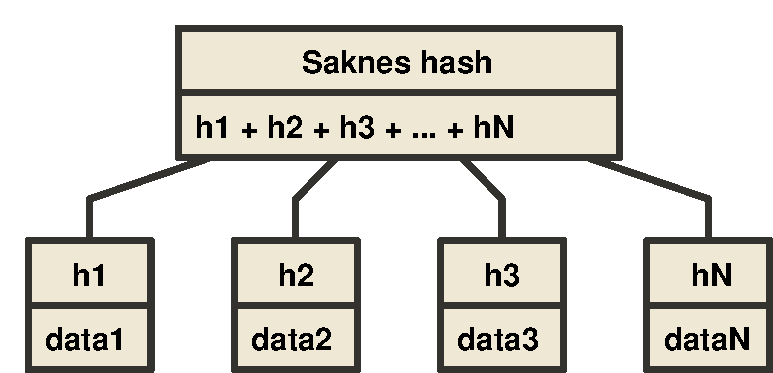
\includegraphics[scale=0.5]{teorija/hash-list.pdf}
    \caption{Hash saraksts}
    Dati tiek sadalīti vairākās daļās katrai daļai tiek aprēķināta hash vērtība. Saknes hash tiek aprēķināts no atsevišķo daļu hash vērtībām.
\label{fig:hash-list}
\end{figure}

Tagad pirms sākt datu ieguvi tiek iegūts saraksts ar hash vērtībām sadalītajiem datiem. Ievēro, ka informācijas apjoms, kas jāpārsūta šajā gadījumā ir ievērojami mazāks par visu datu apjomu. Sarēķina vai hash no saraksta atbilst tam kas tiek iegūts no drošā avota, ja rodas nesakritība, tad ir skaidrs, ka nav vērts sākt pašu datu lejuplādi. Kad ir veiksmīgi iegūts pareizais hash saraksts, tad lejuplādi datiem var veikt no vairākiem avotiem prasot katram avotam savus datu gabaliņus, kā arī uzreiz izķert kļūdas.

Līdzīgi mehānismi tiek izmantoti decentralizētos failu apmaiņas protokolos piemēram BitTorrent. Metode strādā ļoti labi, ja dati laika gaitā ir nemainīgi, tomēr mainīgiem datiem būtu neparocīgi katru reizi pārrēķināt galveno hash vērtību, jo tad tā ir jāmaina uzticamajam avotam. Aplūkosim metodi, kas ļauj ar nemainīgu galveno hash vērtību validēt datus, kuri regulāri tiek pagarināti, bet vēsture paliek nemainīga.

Aplūkojamā datu struktūra sastāv no blokiem, kuri paši sastāv no datiem un iepriekšējā bloka hash vērtības.\cite{nakamoto08} Pats pirmais bloks, kas satur sākotnējo vērtību, nesatur sevī hash vērtību un šo bloku sauc arī par \textit{genesis block}. Datu struktūra ir līdzīga saistītajam sarakstam, bet atšķirība ir tāda, ka nav iespējams mainīt bloka saturu, vai ievietot pa vidu vēl kādu bloku. Skatīt attēlu~\ref{fig:hash-chain}.

\begin{figure}[htpb]
    \centering
    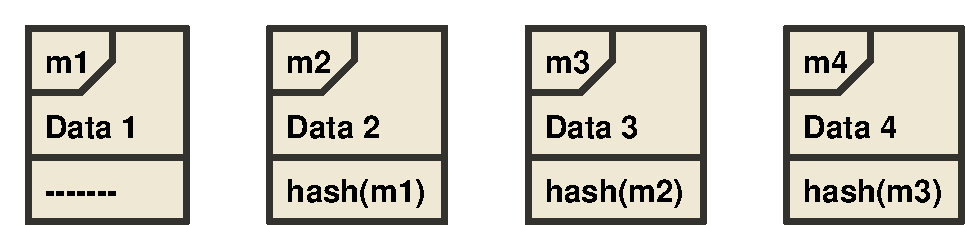
\includegraphics[scale=0.5]{teorija/hash-chain.pdf}
    \caption{Hash ķēde}
    Katrs hash ķēdes ziņojums $m_i$ sastāv no sev raksturīgajiem datiem $d_i$ un
    iepriekšējā posma $m_{i-1}$ hash vērtības.
\label{fig:hash-chain}
\end{figure}

Piemēram, pamainot otrā bloka datu vērtību mainās bloka hash un tas vairs nesakrīt ar trešajā blokā ierakstīto hash vērtību. Savukārt izmainot trešajā blokā ierakstīto otrā bloka hash vērtību izmainās trešā bloka hash, salaužot ceturto bloku. Tātad, lai izmainītu datus blokā $i$ ir jāizmaina visi bloki, kuri seko $i$. Tieši šī datu struktūra tiek izmantota visās blokķēžu implementācijās.

\subsection{Izkliedētā skaitļošana (distributed computing)}
Izkliedētās skaitļošanas pirmssākumi meklējami failu apmaiņā starp vienaudžiem. Mūsdienās populārākais protokols šī mērķa sasniegšanai ir BitTorrent. Ja kāds fails tīklā kļūst populārs, tad ir pamats ticēt, ka tas nevar no turienes pazust, jo veiksmīgākie mēģinājumi cīnīties pret dalīšanos BitTorrent tīklā ir saistīti ar uzbrukumiem tādiem serveriem, kas uztur sarakstu ar tīklā atrodamajiem failiem. Tomēr ir ieviesti strādājoši paplašinājumi BitTorrent protokolam, kas pilda minēto serveru funkciju decentralizētā vidē.\cite{pouwelse08} Tā kā sistēma ir publiski pieejama un noturīga pret cenzūru, tad tā ir piemērota bāze decentralizētas finanšu infrastruktūras radīšanai. Atliek atrisināt problēmu, kur maksājuma pieprasījumiem jābūt vienā secībā, turklāt šī secība nedrīkst mainīties. Tehniskā līmenī ķēde risina tieši šo problēmu.

Piebildīsim, ka ļaundariem paveras jauns uzbrukuma virziens, kas nebija aktuāls BitTorrent gadījumā, jo sistēmā kuru veidojam nedrīkst pieļaut, ka virsotnes ignorē legālas transakcijas, bet no otras puses ļaundaris var uzģenerēt lielu skaitu ar legālām transakcijām, efektīvi veicot DoS uzbrukumu. Vairums ķēžu risina šo problēmu iekasējot nelielu komisiju par katru transakciju.

Aprakstīsim Bizantijas vienošanās problēmu (Byzantine agreement, Byzantine generals problem).
Pieņemsim, ka ir sistēma kas sastāv no tīklā saslēgtiem datoriem, kuri sazinās savā starpā sūtot ziņojumus. Mērķis ir vienoties par koordinētu tālāko rīcību, kas ir atkarīga no ārējiem apstākļiem, kuri iepriekš nav zināmi. Uzdevumu padara grūtu tas, ka starp datoriem var būt arī tādi, kas ļaunprātīgi cenšas sabotēt vienotu rīcību.
Problēmas atrisinājums ir vienprātības algoritms, kuram izpildās divas īpašības.
\begin{enumerate}
    \item Datoram izpildot algoritmu tiek pieņemts tāds pats lēmums, kā citiem datoriem, kuri izpilta algoritmu.
    \item Neliels daudzums ar ļaunprātīgiem datoriem nespēj ietekmēt pieņemto lēmumu.
\end{enumerate}\cite{lamport82}
Turpmāk datoru šīs problēmas kontekstā sauksim par \textbf{virsoni} (node), jo šis termins tiek lietots ar ķēdēm saistītā literatūrā. Veiksim arī citas nelielas modifikācijas dotajam uzdevumam.
Pēc katra pieņemtā lēmuma tīkla stāvoklis būs mainījies un lēmuma pieņemšanu būs nepieciešams atkārtot. Teiksim ka katram pieņemtajam lēmumam $x$ ir indekss $i$. Virsotne var droši \textbf{publicēt} vērtību $x$ pozīcijā $i$, ja visiem iepriekšējiem indeksiem ir publicēts kāds lēmums un virsotne ir pārliecināta, ka arī citas virsotnes laika gaitā publicēs vērtību $x$ pozīcijā $i$.\cite{mazieres15} Tādējādi mēs neprasām, lai visas virsotnes pieņemtu vienotu lēmumu vienlaicīgi, bet gan to, lai vienots lēmums eksistētu. Šāda modifikācija noteikti ir nepieciešama, jo decentralizētā vidē nav pat zināms dalībnieku skaits un viens ļaundaris var netraucēti izlikties par vairākām virsotnēm.
Tādēļ arī otro nosacījumu padarīsim spēcīgāku un skaidrāku, prasot, lai jebkāds daudzums ar ļaunprātīgām virsotnēm nespēj ietekmēt pieņemto lēmumu.
Turklāt kļūst skaidrs, ka mūsu gadījumā demokrātiska lēmuma pieņemšana nav risinājums, tapēc aplūkosim populārākos līdz šim piedāvātos vienprātības algoritmus.

\subsubsection{Pierādījums ar darbu (Proof of work)}
Virsotnes darbojas pēc sekojoša principa:\cite{nakamoto08}
\begin{enumerate}
    \item Jaunās transakcijas tiek paziņotas visām virsotnēm.
    \item Katra virsotne izvēlas transakcijas kuras iekļaut jaunajā blokā.
    \item Katra virotne risina skaitliski sarežģītu problēmu, kas padarītu izvēlēto bloku legālu.
    \item Kad kāda virsotne atrisina problēmu, tad tā paziņo atrasto bloku visām pārējām virsotnēm.
    \item Pārējās virsotnes pārbauda, vai atrastais bloks ir legāls.
    \item Pārējās virsotnes turpina risināt sarežģīto problēmu pa virsu jaunajam blokam.
\end{enumerate}
Trešais punkts nodrošina to, ka ļaundarim nav vērts izlikties par vairākām virsotnēm, jo spēja radīt jaunus blokus ir proporcionāla skaitļošanas jaudai, bet ļaundara skaitļošanas jauda ir ierobežota.

Sesto punktu nepieciešams paskaidrot sīkāk. Par ķēdes \textbf{svaru} sauksim vidējo skaitļošanas darbu, kāds nepieciešams, lai atrastu visus blokus šajā ķēdē. Pareizā vēsture ir tā, kurai ir vislielākais svars. Par bloka atrašanu virsotnes īpašniekam palielinās bilance tapēc visas virsotnes ir motivētas taisīt jaunus blokus uz pareizās vēstures. Kad uz pareizās vēstures tiek atrasts bloks tās svars palielinās un šī vēsture kļūst vēl pareizāka. Ja divām vēsturēm ir līdzīgs svars, tad daļa no virsotnēm meklēs nākamo bloku uz vienas vēstures, bet daļa uz otras. Tai vēsturei, kurai pirmajai atradīs nākamo bloku būs ievērojami lielāks svars un tad visas virsotnes būs motivētas turpināt vienu vēsturi.

Lai ļaundarim izdotos cenzēt transakciju blokā $i$ tad viņam ir jāsāk meklēt bloki sākot no $i-1$ bloka un jāiegulda savā versijā lielāks darbs nekā ir patreizējā vēsturē. Ja ļaundarim ir mazāk kā puse no visu virsotņu skaitļošanas jaudas, tad viņa varbūtība panākt patreizējo vēsturi eksponenciāli dilst atkarībā no attāluma (darba) starp bloku $i-1$ un aktuālo vēsturi.\cite{nakamoto08}

% uzrakstit kkādu diskusiju
\subsubsection{Pierādījums ar risku (Proof of stake)}
\subsubsection{Federatīva Bizantijas vienošanās (FBA)}
Papildināsim uzdevumu ar sekojošajām definīcijām.
\begin{itemize}
    \item 
        Virsotņu kopu sauc par \textbf{drošu}, ja katrām divām virsotnēm tās publicēs vienādas vērtības.
    \item 
        Virsotni sauc par \textbf{dzīvu}, ja spēj publicēt jaunas vērtības nepaļaujoties uz ļaunprātīgo virsotņu sadarbību.
    \item 
        Virsotņu kopu sauc par \textbf{pareizu}, ja tā ir droša un katra virsotne ir dzīva.
\end{itemize}

\begin{figure}[htpb]
    \centering
    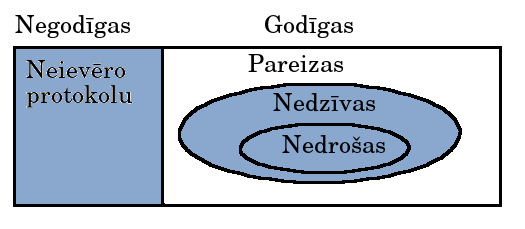
\includegraphics[scale=0.5]{teorija/node-fail.jpg}
    \caption{Venna diagramma virsotņu stāvokļiem}
\label{fig:node-fail}
\end{figure}

\subsubsection{Pierādījums ar DDoS (Proof of DDoS)}

% \begin{description}
%         % torrenti, BGP, consensus nepieciešamība, anti spam nepieciešamība <- parakstu nepieciešamība

% kas ir DA0


\specnodala{Rezultāti}
Tika risināta praktiska problēma kurā uzbrucējs ir nošifrējis upura cieto disku un vēlas apmainīt atšifrēšanas atslēgu pret izpirkuma maksu kriptovalūtā. Tika uzrakstīts kods, kas konceptuālā līmenī demonstrē apmaiņas iespējamību.


\specnodala{Secinājumi}
Līdz ar datoru izveidi kriptogrāfija mainījās no praktiskas disciplīnas par teorētisku zinātni un tās īsajā pastāvēšanas vēsturē attīstība ir notikusi strauji un bez pārtraukumiem. Par blokķēdes pirmsākumiem uzskatāms 2008 gads, kad Satoši Nakamoto uzrakstīja Bitcoin tehnisko aprakstu, tātad tehnoloģija ir pastāvējusi nepilnus 9 gadus. Nopietna pāris simtu lapaspušu grāmata izdota 2015 gadā, kuru izdevās pāršķirstīt radīja iespaidu, ka ir novecojusi un slikti uzrakstīta. Pašlaik priekštatu par blokķēdēm vislabāk gūt no tehniskiem aprakstiem, ierakstiem blogos un informatīviem bukletiem. Augošais un relatīvi vecais kriptovalūtu tirgus liecina, par to, ka blokķēde ir nākotnes tehnoloģija, tomēr augstās maiņas kursa svārstības liecina, ka vēl nav zināms kura no ķēdes realizācijām kļūs par vispārpieņemto standartu. Praktiskas standartizācijas trūkums traucē arī matemātiskas formalizācijas izveidei.

Turpretī godīga apmaiņa ir vecāka un šaurāka problēma, kas ir daudzmaz izpētīta, padarot šo teoriju par labu atspēriena punktu, lai aprakstītu blokķēžu \textit{smart contracts} funkcionalitāti. Ņemot vērā plašo ticību blokķēžu vēstures nemaināmībai ir iespējams praktiski veikt godīgu apmaiņu jebkam, ko ir iespējams `uzlikt' uz ķēdes.

Ķēde ir populārs norēķinu līdzeklis noziedzinieku vidū pateicoties tās pseidonimitātei un necenzējamībai. Efektīvi vienīgais veids, kā aizliegt kriptovalūtas ir ar smagu interneta cenzūru.


\specnodala{Pateicības}
\begin{itemize}
    \item Viktorijai Leimanei par valodas salabošanu.
    \item GNU projektam par kvalitatīvajiem rīkiem, kas palīdzēja darba tapšanā.
    \item Jānim Valeinim par \LaTeX{} stila izstrādi.
\end{itemize}


\literatura{main}

\appendix
\chapter{Izveidoto programmu kods}
not implemented

\end{document}
